% Options for packages loaded elsewhere
% Options for packages loaded elsewhere
\PassOptionsToPackage{unicode}{hyperref}
\PassOptionsToPackage{hyphens}{url}
\PassOptionsToPackage{dvipsnames,svgnames,x11names}{xcolor}
%
\documentclass[
  12pt,
  letterpaper,
  number]{elsarticle}
\usepackage{xcolor}
\usepackage{amsmath,amssymb}
\setcounter{secnumdepth}{5}
\usepackage{iftex}
\ifPDFTeX
  \usepackage[T1]{fontenc}
  \usepackage[utf8]{inputenc}
  \usepackage{textcomp} % provide euro and other symbols
\else % if luatex or xetex
  \usepackage{unicode-math} % this also loads fontspec
  \defaultfontfeatures{Scale=MatchLowercase}
  \defaultfontfeatures[\rmfamily]{Ligatures=TeX,Scale=1}
\fi
\usepackage{lmodern}
\ifPDFTeX\else
  % xetex/luatex font selection
\fi
% Use upquote if available, for straight quotes in verbatim environments
\IfFileExists{upquote.sty}{\usepackage{upquote}}{}
\IfFileExists{microtype.sty}{% use microtype if available
  \usepackage[]{microtype}
  \UseMicrotypeSet[protrusion]{basicmath} % disable protrusion for tt fonts
}{}
\makeatletter
\@ifundefined{KOMAClassName}{% if non-KOMA class
  \IfFileExists{parskip.sty}{%
    \usepackage{parskip}
  }{% else
    \setlength{\parindent}{0pt}
    \setlength{\parskip}{6pt plus 2pt minus 1pt}}
}{% if KOMA class
  \KOMAoptions{parskip=half}}
\makeatother
% Make \paragraph and \subparagraph free-standing
\makeatletter
\ifx\paragraph\undefined\else
  \let\oldparagraph\paragraph
  \renewcommand{\paragraph}{
    \@ifstar
      \xxxParagraphStar
      \xxxParagraphNoStar
  }
  \newcommand{\xxxParagraphStar}[1]{\oldparagraph*{#1}\mbox{}}
  \newcommand{\xxxParagraphNoStar}[1]{\oldparagraph{#1}\mbox{}}
\fi
\ifx\subparagraph\undefined\else
  \let\oldsubparagraph\subparagraph
  \renewcommand{\subparagraph}{
    \@ifstar
      \xxxSubParagraphStar
      \xxxSubParagraphNoStar
  }
  \newcommand{\xxxSubParagraphStar}[1]{\oldsubparagraph*{#1}\mbox{}}
  \newcommand{\xxxSubParagraphNoStar}[1]{\oldsubparagraph{#1}\mbox{}}
\fi
\makeatother


\usepackage{longtable,booktabs,array}
\usepackage{calc} % for calculating minipage widths
% Correct order of tables after \paragraph or \subparagraph
\usepackage{etoolbox}
\makeatletter
\patchcmd\longtable{\par}{\if@noskipsec\mbox{}\fi\par}{}{}
\makeatother
% Allow footnotes in longtable head/foot
\IfFileExists{footnotehyper.sty}{\usepackage{footnotehyper}}{\usepackage{footnote}}
\makesavenoteenv{longtable}
\usepackage{graphicx}
\makeatletter
\newsavebox\pandoc@box
\newcommand*\pandocbounded[1]{% scales image to fit in text height/width
  \sbox\pandoc@box{#1}%
  \Gscale@div\@tempa{\textheight}{\dimexpr\ht\pandoc@box+\dp\pandoc@box\relax}%
  \Gscale@div\@tempb{\linewidth}{\wd\pandoc@box}%
  \ifdim\@tempb\p@<\@tempa\p@\let\@tempa\@tempb\fi% select the smaller of both
  \ifdim\@tempa\p@<\p@\scalebox{\@tempa}{\usebox\pandoc@box}%
  \else\usebox{\pandoc@box}%
  \fi%
}
% Set default figure placement to htbp
\def\fps@figure{htbp}
\makeatother


% definitions for citeproc citations
\NewDocumentCommand\citeproctext{}{}
\NewDocumentCommand\citeproc{mm}{%
  \begingroup\def\citeproctext{#2}\cite{#1}\endgroup}
\makeatletter
 % allow citations to break across lines
 \let\@cite@ofmt\@firstofone
 % avoid brackets around text for \cite:
 \def\@biblabel#1{}
 \def\@cite#1#2{{#1\if@tempswa , #2\fi}}
\makeatother
\newlength{\cslhangindent}
\setlength{\cslhangindent}{1.5em}
\newlength{\csllabelwidth}
\setlength{\csllabelwidth}{3em}
\newenvironment{CSLReferences}[2] % #1 hanging-indent, #2 entry-spacing
 {\begin{list}{}{%
  \setlength{\itemindent}{0pt}
  \setlength{\leftmargin}{0pt}
  \setlength{\parsep}{0pt}
  % turn on hanging indent if param 1 is 1
  \ifodd #1
   \setlength{\leftmargin}{\cslhangindent}
   \setlength{\itemindent}{-1\cslhangindent}
  \fi
  % set entry spacing
  \setlength{\itemsep}{#2\baselineskip}}}
 {\end{list}}
\usepackage{calc}
\newcommand{\CSLBlock}[1]{\hfill\break\parbox[t]{\linewidth}{\strut\ignorespaces#1\strut}}
\newcommand{\CSLLeftMargin}[1]{\parbox[t]{\csllabelwidth}{\strut#1\strut}}
\newcommand{\CSLRightInline}[1]{\parbox[t]{\linewidth - \csllabelwidth}{\strut#1\strut}}
\newcommand{\CSLIndent}[1]{\hspace{\cslhangindent}#1}



\setlength{\emergencystretch}{3em} % prevent overfull lines

\providecommand{\tightlist}{%
  \setlength{\itemsep}{0pt}\setlength{\parskip}{0pt}}



 


% These are extra latex packages that the document depends on
% 
\usepackage[margin=1in]{geometry}
\usepackage{siunitx}
\usepackage{tabularray}
\UseTblrLibrary{siunitx}
\usepackage{fontspec}

\setmainfont{Times New Roman}
\usepackage{booktabs}
\usepackage{longtable}
\usepackage{array}
\usepackage{multirow}
\usepackage{wrapfig}
\usepackage{float}
\usepackage{colortbl}
\usepackage{pdflscape}
\usepackage{tabularx}
\usepackage{xltabular}
\usepackage{threeparttable}
\usepackage{threeparttablex}
\usepackage[normalem]{ulem}
\usepackage{makecell}
\usepackage{xcolor}
\makeatletter
\@ifpackageloaded{bookmark}{}{\usepackage{bookmark}}
\makeatother
\makeatletter
\@ifpackageloaded{caption}{}{\usepackage{caption}}
\AtBeginDocument{%
\ifdefined\contentsname
  \renewcommand*\contentsname{Table of contents}
\else
  \newcommand\contentsname{Table of contents}
\fi
\ifdefined\listfigurename
  \renewcommand*\listfigurename{List of Figures}
\else
  \newcommand\listfigurename{List of Figures}
\fi
\ifdefined\listtablename
  \renewcommand*\listtablename{List of Tables}
\else
  \newcommand\listtablename{List of Tables}
\fi
\ifdefined\figurename
  \renewcommand*\figurename{Figure}
\else
  \newcommand\figurename{Figure}
\fi
\ifdefined\tablename
  \renewcommand*\tablename{Table}
\else
  \newcommand\tablename{Table}
\fi
}
\@ifpackageloaded{float}{}{\usepackage{float}}
\floatstyle{ruled}
\@ifundefined{c@chapter}{\newfloat{codelisting}{h}{lop}}{\newfloat{codelisting}{h}{lop}[chapter]}
\floatname{codelisting}{Listing}
\newcommand*\listoflistings{\listof{codelisting}{List of Listings}}
\makeatother
\makeatletter
\makeatother
\makeatletter
\@ifpackageloaded{caption}{}{\usepackage{caption}}
\@ifpackageloaded{subcaption}{}{\usepackage{subcaption}}
\makeatother
\journal{ASCE 2027}
\usepackage{bookmark}
\IfFileExists{xurl.sty}{\usepackage{xurl}}{} % add URL line breaks if available
\urlstyle{same}
\hypersetup{
  pdftitle={Effectiveness of Temporary Portable Rumble Strips in Utah},
  pdfauthor={Gregory S. Macfarlane; Tyler Carruth; Benjamin Hailstone; Grant Schultz},
  colorlinks=true,
  linkcolor={blue},
  filecolor={Maroon},
  citecolor={Blue},
  urlcolor={Blue},
  pdfcreator={LaTeX via pandoc}}


\setlength{\parindent}{6pt}
\begin{document}

\begin{frontmatter}
\title{Effectiveness of Temporary Portable Rumble Strips in Utah}
\author[1]{Gregory S. Macfarlane%
%
}
 \ead{gregmacfarlane@byu.edu} 
\author[1]{Tyler Carruth%
%
}

\author[1]{Benjamin Hailstone%
%
}

\author[1]{Grant Schultz%
%
}


\affiliation[1]{organization={Civil and Construction Engineering
Department, Brigham Young University},addressline={430
EB},city={Provo},postcode={84602},postcodesep={}}

\cortext[cor1]{Corresponding author}




        
\begin{abstract}
This study evaluates the effectiveness and operational implications of
Temporary Portable Rumble Strips (TPRS) used by the Utah Department of
Transportation (UDOT) to alert drivers to upcoming work zones. While
TPRS are intended to capture driver attention and reduce crash risk,
concerns remain regarding their influence on driver behavior, avoidance
maneuvers, and maintenance requirements. A field experiment was
conducted at four work zones in Utah during the Summer 2025 construction
season. Four deployment conditions---no TPRS and three spacing
configurations---were tested. Data collection included speed
measurements using mobile radar detectors and video-based observations
of vehicle classification, braking behavior, avoidance maneuvers, and
TPRS displacement. Results indicate that the effect of TPRS on speed
reduction is inconclusive. Drivers who braked in response to TPRS
typically did so before reaching the devices, suggesting that visual
cues may be as influential as tactile feedback. Avoidance behavior was
common among motorcycles and occurred occasionally among other vehicles.
Driver responses were more strongly influenced by site-specific
factors---such as roadway geometry and sight distance---than by TPRS
spacing. TPRS displacement occurred gradually under traffic but was not
clearly related to traffic volume or speed, suggesting that device age
and condition play a larger role. Maintenance requires traffic gaps of
approximately 34 seconds, which may not be feasible at higher-volume
sites. These findings highlight the need for further evaluation of TPRS
effectiveness, standards for device condition, consideration of
alternative measures for long-term work zones, and increased contractor
discretion based on site conditions.
\end{abstract}





\end{frontmatter}
    

\bookmarksetup{startatroot}

\section{Introduction}\label{sec-intro}

Temporary portable rumble strips (TPRS) have been used since at least
the early 2000s to alert drivers to upcoming work zones. These devices
are made of steel and rubber and are placed transverse across the
roadway in arrays of strips (Meyer et al., 2006; PSS, 2018).

At the same time, TPRS introduces additional complication in work zones.
Workers must enter the roadway to install the strips and adjust them
when they become displaced. Anecdotal evidence suggests that some
drivers may avoid TPRS, creating a safety hazard. And as drivers become
accustomed to strips, they may become desensitized to them, making them
less effective.

In this research, we report a field experiment to evaluate driver
reaction to TPRS and observe

This paper is organized as follows: First, a Literature Review section
briefly outlines previous research results in TPRS. A Methodology
sections describes the experimental design and methods used to collect
data, with a subsequent Results section presenting the results of the
experiment. A final Conclusion section discusses the implications of the
findings for practice and future research.

\bookmarksetup{startatroot}

\section{Literature Review}\label{literature-review}

\subsection{Overview}\label{overview}

Non-adhesive TPRS, typically made of steel and rubber, have been used
since 2009 to improve work zone safety (\textbf{pss\_best\_2018?}).
Research consistently shows that TPRS can reduce traffic speed, increase
driver attentiveness, and minimize erratic driving behaviors such as
lane departures (\textbf{yang\_effectiveness\_2015?}).

\subsection{Speed Reduction}\label{speed-reduction}

TPRS installations are effective at reducing vehicle speeds in work
zones. Studies report speed reductions ranging from 3.5 to 13.8
mph,(\textbf{yang\_effectiveness\_2015?}), with greater reductions
observed near the first set of strips and when drivers can see a flagger
or additional barriers (\textbf{wang\_effects\_2013?}).
(\textbf{wang\_effects\_2013?}) shows the effect is highly localized,
and speeds tend to increase once drivers pass the TPRS unless additional
measures are present.

\subsection{Driver Behavior}\label{driver-behavior}

TPRS increase driver attentiveness, often measured by the frequency of
brake light activation as vehicles approach the strips. Studies show
that TPRS prompt more drivers to brake and pay attention to changing
road conditions, though the percentage varies from 11 perecnt to 55
percent based on site and conditions
(\textbf{brown\_effectiveness\_2022?};
\textbf{sun\_elevated-risk\_2011?}; \textbf{wang\_effects\_2013?};
\textbf{yang\_effectiveness\_2015?}). Commercial vehicles tend to
respond more cautiously than passenger cars
(\textbf{wang\_effects\_2013?}).

Concerns about drivers evading TPRS by leaving their lane have been
largely unfounded. Most studies report minimal lane departures,
especially when TPRS are installed across the full width of the road
(\textbf{sun\_elevated-risk\_2011?}; \textbf{wang\_effects\_2013?};
\textbf{brown\_effectiveness\_2022?}). Lane departures are more likely
on narrow roads or near the end of a TPRS array, but overall rates are
low (\textbf{sun\_elevated-risk\_2011?}).

\subsection{TPRS Displacement}\label{tprs-displacement}

A key challenge with non-adhesive TPRS is their tendency to shift or
become displaced under traffic. Displacement increases with heavier
vehicles, higher speeds, and higher traffic volume
(\textbf{sun\_elevated-risk\_2011?}). Placement angle also
matters---strips that rotate away from perpendicular to traffic tend to
move more(\textbf{sun\_elevated-risk\_2011?}). Real-world studies show
that while displacement is generally manageable, it can require periodic
adjustment, which may increase worker exposure to traffic. The effect of
strip wear and long-term durability under heavy use is not well
understood and requires further research.

\subsection{Spacing Specifications}\label{spacing-specifications}

There are three main groups of spacing specifications. Some states, such
as Wisconsin, Florida, and Colorado, specify a single spacing
independent of speed (e.g., W. DOT, 2022). Some states such as Maryland,
Viriginia, Minnesota, and Utah vary spacing from 10 to 20 ft. based on
the posted speed limit (M. DOT, 2024). New York, Texas, and Missouri
specify spacing from 10 to 35 ft. based on the posted speed
limit(\textbf{citation?}). The manufacturer also recommends spacing of
10 to 35 ft. based on the posted speed limit(\textbf{citation?}). The
various specifications are shown in Figure Figure~\ref{fig-state-specs}.

\begin{figure}

\centering{

\pandocbounded{\includegraphics[keepaspectratio]{02_litreview_files/figure-pdf/fig-state-specs-1.pdf}}

}

\caption{\label{fig-state-specs}Various specifications for TPRS
spacing.}

\end{figure}%

\subsection{Summary}\label{summary}

TPRS are effective at reducing speeds, increasing driver attentiveness,
and minimizing erratic driving in work zones. Displacement under traffic
remains a practical concern, especially for non-adhesive products, and
more research is needed on long-term performance and optimal deployment
strategies.

\bookmarksetup{startatroot}

\section{Methodology}\label{sec-methodology}

This chapter describes the methodology designed by the research team to
evaluate the effectiveness, durability, and stability of TPRS systems on
high-speed roadways in Utah. The experiment will observe driver behavior
and TPRS displacement under traffic load. Cameras and Wavetronix units
will be used to collect the desired data. The designed experiment will
observe the results that occur in the absence of TPRS and in layouts
that vary the spacing between the individual strips in arrays. The
experiment will be designed to maximize observation time and minimize
how often contractors will need to adjust the TPRS. Work sites were
selected for observation based on traffic volume, availability, and
location.

\subsection{Site Selection}\label{site-selection}

The team selected work sites available during the summer of 2025 based
on their driving distance from Provo. The research team used 2023 AADT
data to estimate how many vehicles typically traveled on each road
segment associated with a work site being considered for observation.
This estimate ensured that the roads chosen for observation had enough
traffic to support a reliable statistical analysis of the potential
effect spacing would have on TPRS arrays.

\begin{figure}

\centering{

\pandocbounded{\includegraphics[keepaspectratio]{03_methods_files/figure-pdf/fig-map-1.pdf}}

}

\caption{\label{fig-map}Map of sites}

\end{figure}%

\begin{table}

\caption{\label{tbl-sites}Data Collection Sites}

\centering{

\centering
\begin{tblr}[         %% tabularray outer open
]                     %% tabularray outer close
{                     %% tabularray inner open
colspec={Q[]Q[]Q[]Q[]Q[]},
hline{2}={1-5}{solid, black, 0.05em},
hline{1}={1-5}{solid, black, 0.08em},
hline{6}={1-5}{solid, black, 0.08em},
}                     %% tabularray inner close
Site & Roadway & Location & Start & End \\
1 & SR-12 & Mile marker 6.5 & 2025-07-07 & 2025-07-11 \\
2 & US-6 & 20 miles W of Wellington & 2025-07-15 & 2025-07-18 \\
3 & I-70 & Clear Creek Summit & 2025-07-29 & 2025-08-01 \\
4 & US-191 & North of summit & 2025-08-05 & 2025-08-08 \\
\end{tblr}

}

\end{table}%

The research team used histograms of haverage hourly volumes on Utah
roads to determine which ones would make reliable sites to study to
ensure statistical significance. Figure~\ref{fig-aadt} shows data from
four counting stations near the sites selected for observation. Volume
data from May 2023 to August 2023 was collected from the UDOT Traffic
Data Portal, aggregated and averaged by hour, and plotted as histograms.
The data shows that the sites selected for observation have a sufficient
volume of traffic to support a reliable statistical analysis of the
potential effect spacing would have on TPRS arrays.

\begin{figure}

\centering{

\pandocbounded{\includegraphics[keepaspectratio]{03_methods_files/figure-pdf/fig-aadt-1.pdf}}

}

\caption{\label{fig-aadt}Histogram of average hourly volumes from
counting stations near sites.}

\end{figure}%

\subsection{Layouts}\label{layouts}

The team designed layouts to test the effectiveness of TPRS at work
sites. These layouts were set up at the arrays of TPRS positioned in
front of each work site preceding the tapering line of cones that marked
the beginning of the work zone. Each layout consisted of two Wavetronix
radar detectors and two countCAM4 cameras from StreetLogic Pro. These
devices were mounted on trailers and tripods stationed on the side of
the road. The layouts are depicted below, showing the set-ups designed
for both single-lane and passing-lane configurations.

\begin{center}
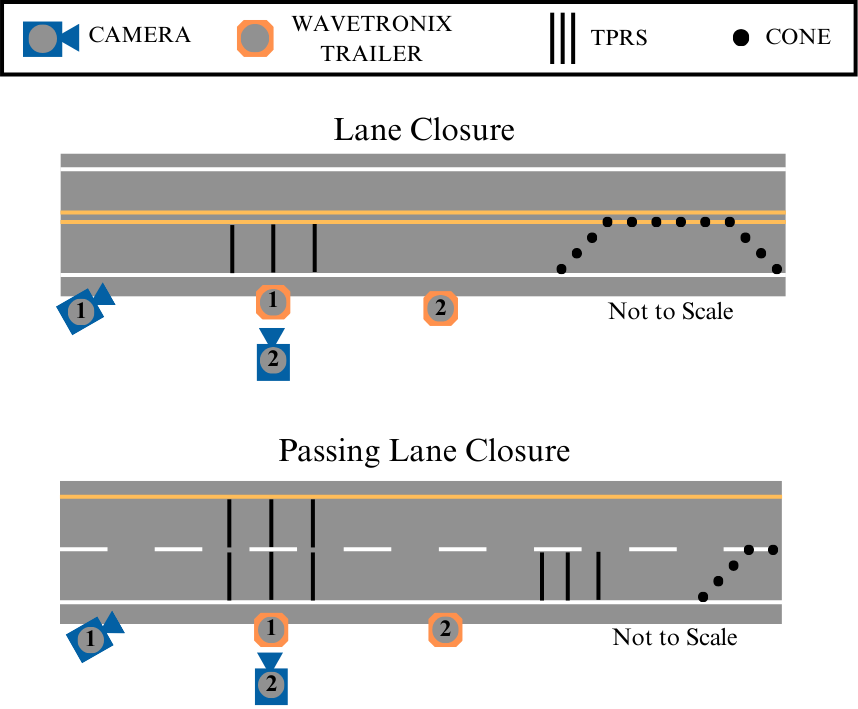
\includegraphics[width=7in,height=\textheight,keepaspectratio]{methodology-diagram.png}
\end{center}

The research team primarily focused on testing the space between
individual TPRS to observe its effect on driver speed and behavior. They
also examined whether the strips could remain in place without requiring
frequent readjustments. The team developed a spacing system for
contractors to use during observation days, tailored to the posted speed
limit at each site. The different spacing specifications, shown in
Figure~\ref{fig-test-spacing} were derived from current UDOT standards
for TPRS spacing and an unofficial rule of thumb from Plastic Safety
Systems (PSS) for their RoadQuake TPRS system.

\begin{figure}

\centering{

\pandocbounded{\includegraphics[keepaspectratio]{03_methods_files/figure-pdf/fig-test-spacing-1.pdf}}

}

\caption{\label{fig-test-spacing}Spacing specifications used in
testing.}

\end{figure}%

\begin{table}

\caption{\label{tbl-wav-spacing}Separation {[}ft{]} Between Wavetronix
Units}

\centering{

\centering
\begin{tblr}[         %% tabularray outer open
]                     %% tabularray outer close
{                     %% tabularray inner open
colspec={Q[]Q[]Q[]Q[]Q[]},
hline{2}={1-5}{solid, black, 0.05em},
hline{1}={1-5}{solid, black, 0.08em},
hline{6}={1-5}{solid, black, 0.08em},
}                     %% tabularray inner close
Site & UDOT & NO TPRS & 1:2 & LONG \\
SR-12 & 762/875 & 851 & 878 & 898 \\
US-6 & 516 & 516 & 516 & 516 \\
I-70 & 800 & 804 & 782 & 765 \\
US-191 & 782 & 748 & 781 & 759 \\
\end{tblr}

}

\end{table}%

\subsection{Driver Behavior - Change in Speed, Braking, and Lane
Departures}\label{driver-behavior---change-in-speed-braking-and-lane-departures}

The research team observed driver behavior by analyzing the data
collected from the Wavetronix radar detectors and StreetLogic Pro
cameras. The Wavetronix units provided data on vehicle speed and braking
patterns, while the cameras captured footage to identify lane departures
and other driving behaviors. The team compared these behaviors across
different spacing configurations to assess the effectiveness of TPRS in
influencing driver behavior in work zones.

\subsection{TPRS Displacement and Worker
Exposure}\label{tprs-displacement-and-worker-exposure}

\begin{center}
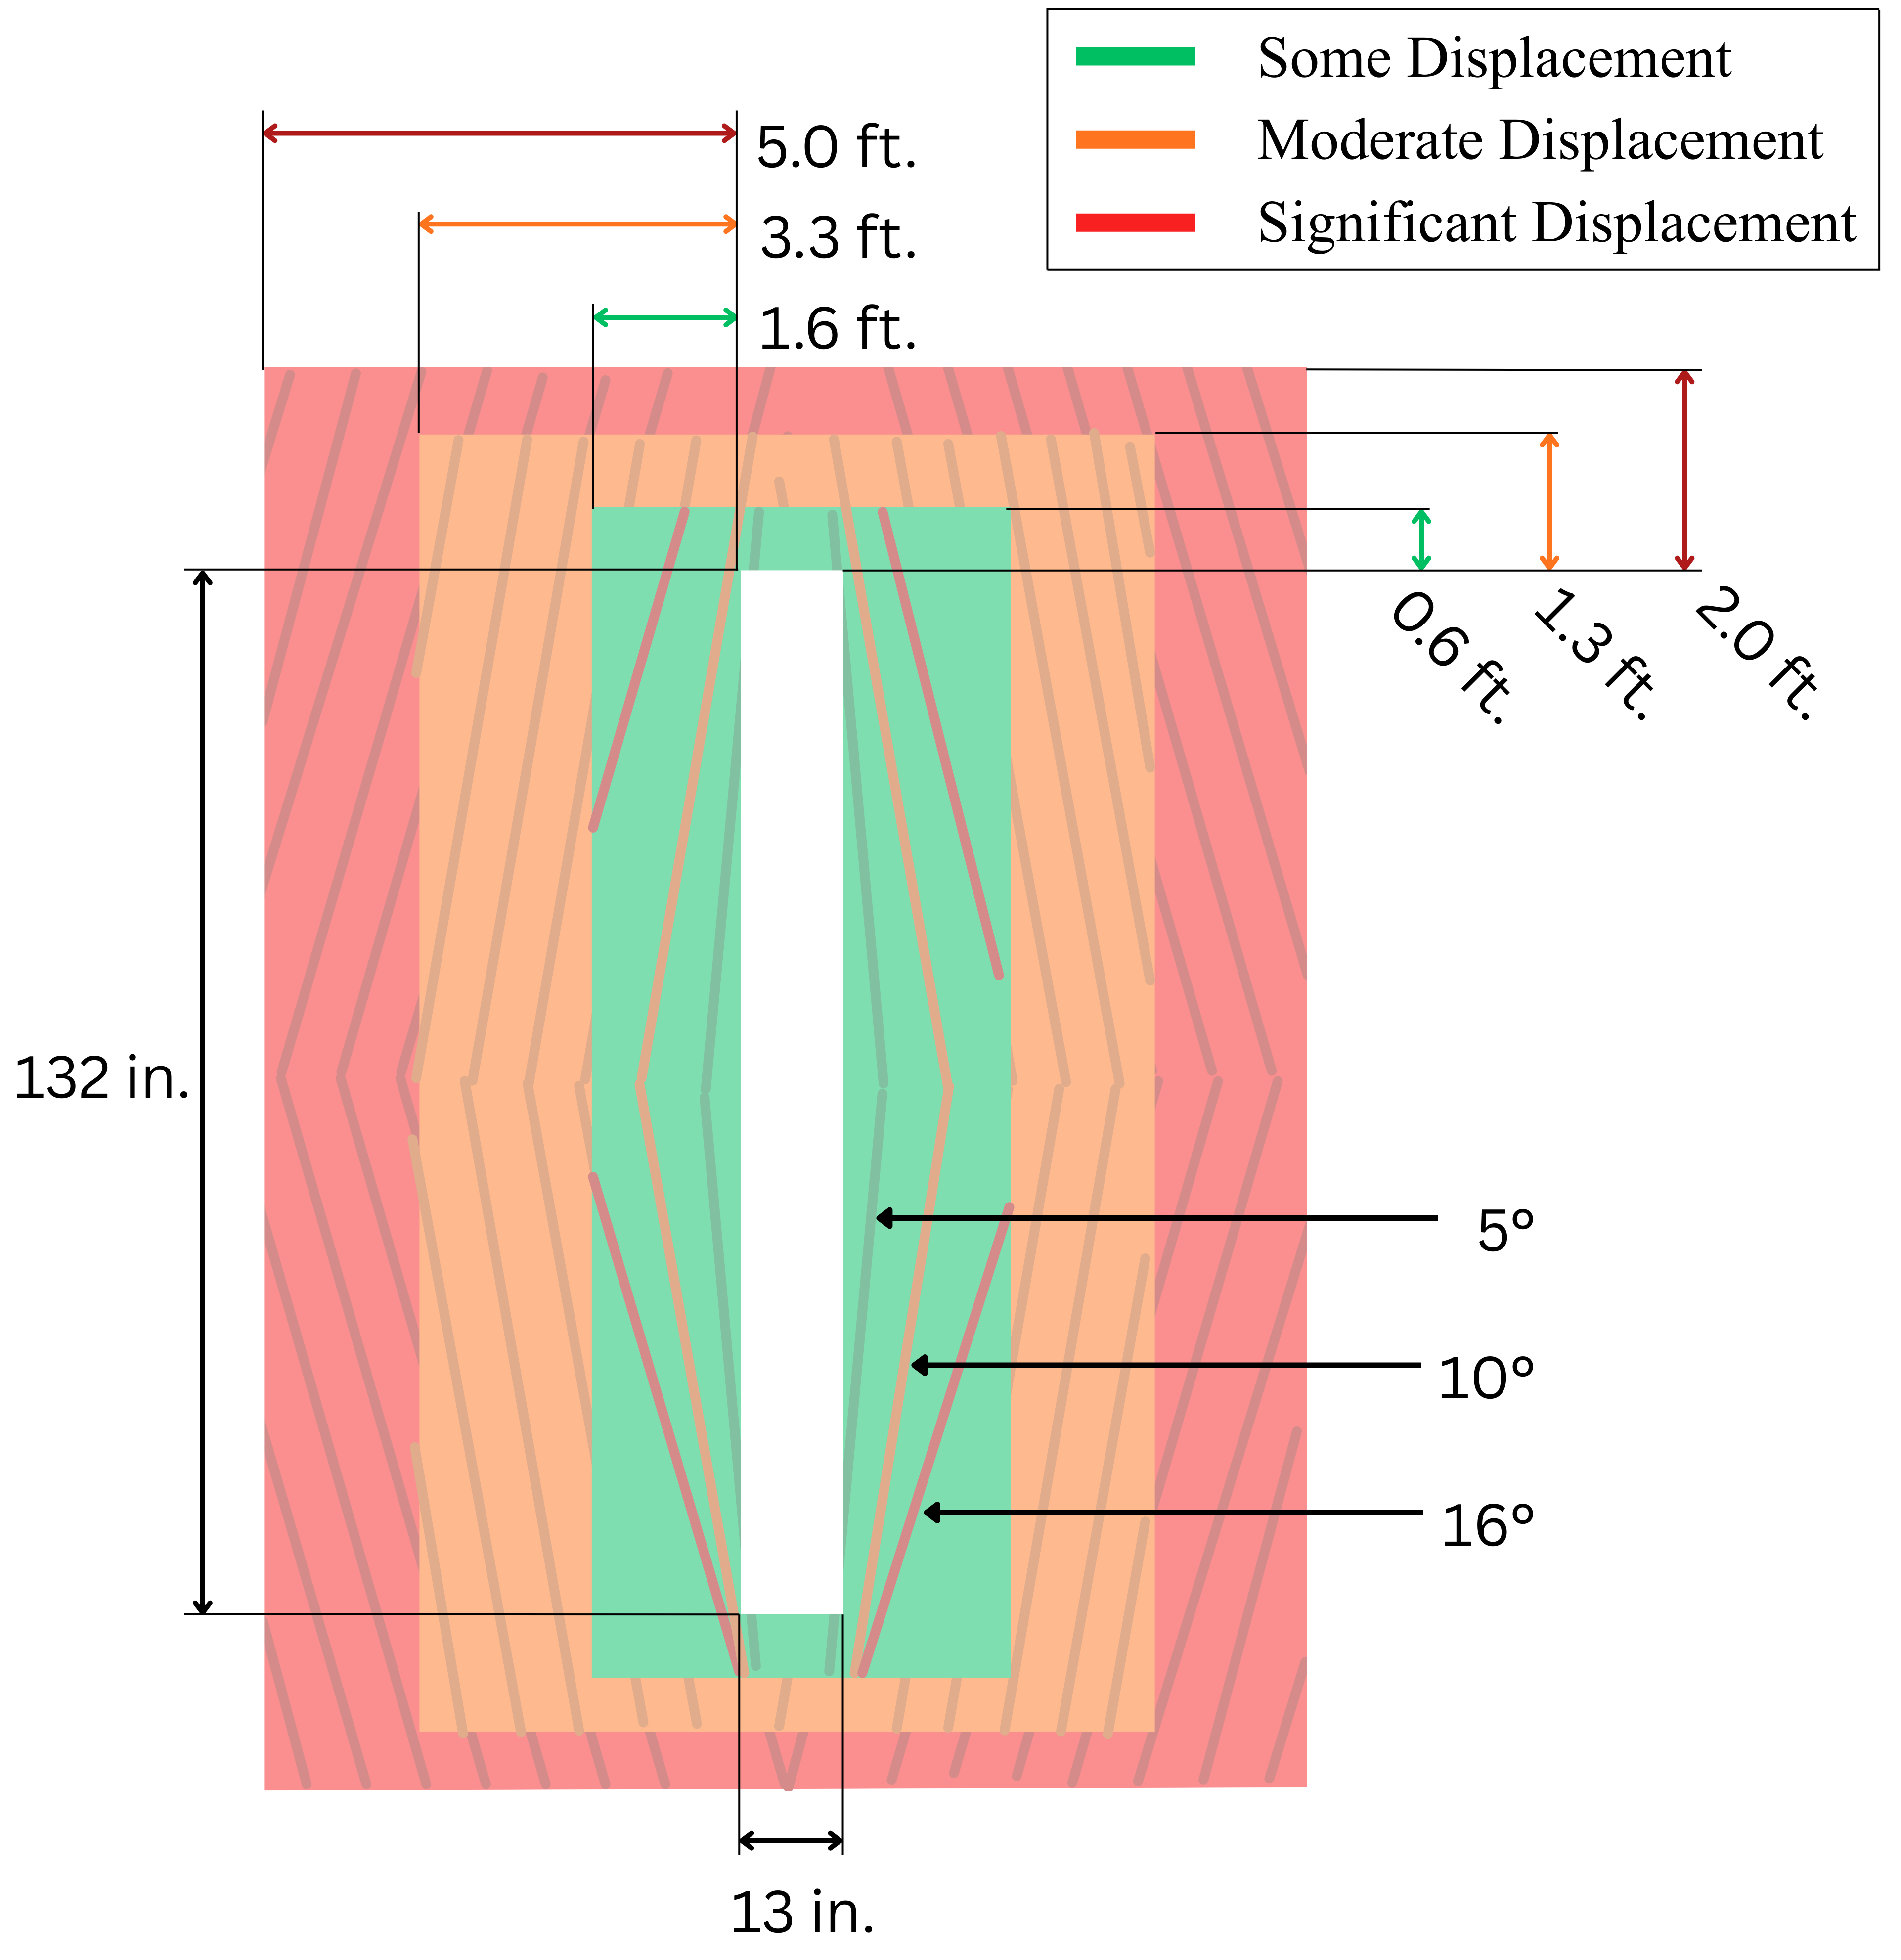
\includegraphics[width=7in,height=\textheight,keepaspectratio]{displacement_overlay.png}
\end{center}

\begin{center}
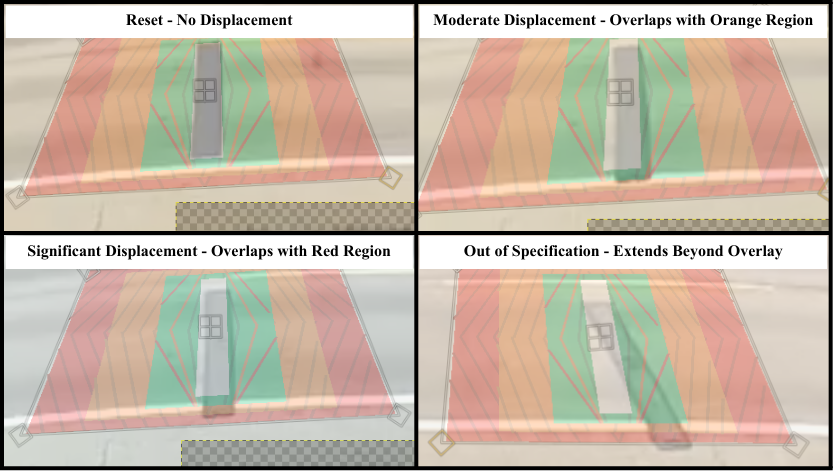
\includegraphics[width=7in,height=\textheight,keepaspectratio]{examples-of-displacement.png}
\end{center}

\bookmarksetup{startatroot}

\section{Results and Analysis}\label{sec-results}

This section presents the results of the methodology in
Chapter~\ref{sec-methodology}.

\subsection{Speeds}\label{speeds}

Figure~\ref{fig-speed} shows the change in speed between units, 95\%
confidence bound of different between 85th percentile speeds. The 95\%
confidence bound is the range of speeds that are likely to occur if the
null hypothesis is true. The confidence bounds are calculated using the
bootstrap method. The 95\% confidence bound is calculated by taking the
upper and lower bounds of the 95\% confidence interval, and then taking
the difference between them. This is a useful metric for understanding
the effect of rumble strips on traffic flow.

\begin{figure}

\centering{

\pandocbounded{\includegraphics[keepaspectratio]{04_results_files/figure-pdf/fig-speed-1.pdf}}

}

\caption{\label{fig-speed}Change in speed between units, 95\% confidence
bound of different between 85th percentile speeds.}

\end{figure}%

\subsection{Braking Behavior}\label{braking-behavior}

\subsection{Avoidance Behavior}\label{avoidance-behavior}

\begin{figure}

\centering{

\pandocbounded{\includegraphics[keepaspectratio]{04_results_files/figure-pdf/fig-avoidance-1.pdf}}

}

\caption{\label{fig-avoidance}Avoidance behavior by spacing of TPRS and
vehicle type.}

\end{figure}%

\begin{table}

\caption{\label{tbl-avoidglm}Binomial Models of TPRS Avoidance}

\centering{

\centering
\begin{talltblr}[         %% tabularray outer open
entry=none,label=none,
note{}={+ p \num{< 0.1}, * p \num{< 0.05}, ** p \num{< 0.01}, *** p \num{< 0.001}},
]                     %% tabularray outer close
{                     %% tabularray inner open
colspec={Q[]Q[]Q[]Q[]Q[]Q[]},
hline{2}={1-6}{solid, black, 0.05em},
hline{20}={1-6}{solid, black, 0.05em},
hline{1}={1-6}{solid, black, 0.08em},
hline{25}={1-6}{solid, black, 0.08em},
column{2-6}={}{halign=c},
column{1}={}{halign=l},
}                     %% tabularray inner close
& Pooled & SR-12 & US-6 & I-70 & US-191 \\
(Intercept) & -7.852*** & -5.622*** & -7.577*** & -21.499 & -6.343*** \\
& (0.382) & (0.413) & (1.012) & (754.412) & (1.009) \\
Trucks & 0.166 & 0.306 & 0.536 & -0.669+ & 0.121 \\
& (0.117) & (0.204) & (0.364) & (0.388) & (0.172) \\
Motorcycles & 2.213*** & 2.192*** & 2.874*** & 3.836*** & 2.060*** \\
& (0.210) & (0.282) & (0.777) & (0.948) & (0.354) \\
UDOT Spacing & 3.189*** & 2.868*** & 1.875+ & 16.662 & 4.313*** \\
& (0.367) & (0.433) & (1.063) & (754.413) & (1.013) \\
1:2 Spacing & 3.538*** & 3.092*** & 3.145** & 17.971 & 4.312*** \\
& (0.363) & (0.423) & (1.043) & (754.412) & (1.012) \\
Long Spacing & 3.292*** & 3.165*** & 2.723** & 15.184 & 4.071*** \\
& (0.365) & (0.424) & (1.030) & (754.413) & (1.016) \\
SR-12 & 1.947*** &  &  &  &  \\
& (0.153) &  &  &  &  \\
US-191 & 2.352*** &  &  &  &  \\
& (0.165) &  &  &  &  \\
US-6 & -0.332 &  &  &  &  \\
& (0.213) &  &  &  &  \\
Num.Obs. & 19016 & 4963 & 6324 & 5933 & 1796 \\
AIC & 4056.3 & 2018.0 & 454.8 & 530.1 & 1022.9 \\
BIC & 4126.9 & 2057.1 & 495.3 & 570.2 & 1055.9 \\
Log.Lik. & -2019.131 & -1003.004 & -221.398 & -259.041 & -505.462 \\
RMSE & 0.16 & 0.23 & 0.08 & 0.09 & 0.28 \\
\end{talltblr}

}

\end{table}%

\subsubsection{Strip Displacement}\label{strip-displacement}

\begin{figure}

\centering{

\pandocbounded{\includegraphics[keepaspectratio]{04_results_files/figure-pdf/fig-momentum-site-1.pdf}}

}

\caption{\label{fig-momentum-site}Impact momentum for each transition,
colored by site.}

\end{figure}%

\begin{figure}

\centering{

\pandocbounded{\includegraphics[keepaspectratio]{04_results_files/figure-pdf/fig-momentum-spacing-1.pdf}}

}

\caption{\label{fig-momentum-spacing}Impact momentum for each
transition, colored by spacing.}

\end{figure}%

Figure~\ref{fig-momentum-site} shows the impact momentum for each
transition, colored by site. The impact momentum is the change in speed
for a vehicle in a given transition. The change in speed is calculated
by subtracting the speed at the beginning of the transition from the
speed at the end of the transition. This is a useful metric for
understanding the effect of rumble strips on traffic flow.

\subsubsection{Worker Exposure}\label{worker-exposure}

\begin{figure}

\centering{

\pandocbounded{\includegraphics[keepaspectratio]{04_results_files/figure-pdf/fig-cdf-1.pdf}}

}

\caption{\label{fig-cdf}CDF of headways for each site.}

\end{figure}%

\bookmarksetup{startatroot}

\section{Conclusions}\label{conclusions}

This section need not be overly long. You should address any limitations
of your results, such as dependence on underlying assumptions or
geographic scope. You should also provide a map for future research.

Finally, you should underline the contributions of this work and any
practical relevance.

\bookmarksetup{startatroot}

\section*{References}\label{references}
\addcontentsline{toc}{section}{References}

\markboth{References}{References}

\phantomsection\label{refs}
\begin{CSLReferences}{1}{0}
\bibitem[\citeproctext]{ref-minnesotadot38278186LongTerm2024}
DOT, M. (2024). \emph{38278186 - {Long Term TTC Layout} for {Two-Lane},
{Two-Way}}.
https://edocs-public.dot.state.mn.us/edocs\_public/DMResultSet/Urlsearch?columns=docnumber,docname\&folderid=38278186\&currSortFieldName=docname\&sortOrder=d.

\bibitem[\citeproctext]{ref-wisconsindotWisconsinDepartmentTransportation2022}
DOT, W. (2022). Wisconsin {Department} of {Transportation Standard
Detail Drawings} ({SDDs}). In \emph{Wisconsin.gov}.
https://wisconsindot.gov/Pages/doing-bus/eng-consultants/cnslt-rsrces/rdwy/sdd.aspx.

\bibitem[\citeproctext]{ref-meyerDesignPortableRumble2006}
Meyer, E., Hale, R., Taghavi, R., Olafsen, J., \& Mathur, G. (2006).
\emph{Design of {Portable Rumble Strips}, {Phase} 2}. InTrans.

\bibitem[\citeproctext]{ref-pssBestPracticesOptimal2018}
PSS. (2018). \emph{{Best Practices for Optimal Use 2nd Edition -
RoadQuake Temporary Portable Rumble Strip}}.

\end{CSLReferences}




\end{document}
